\documentclass[border=10pt]{standalone}

\usepackage{tikz}
\usepackage{tikzsymbols}
\usetikzlibrary{calc,patterns,shapes.geometric}

\def\centerarc[#1](#2)(#3:#4:#5){\draw[#1] ($(#2)+({#5*cos(#3)},{#5*sin(#3)})$) arc (#3:#4:#5);}

\begin{document}
	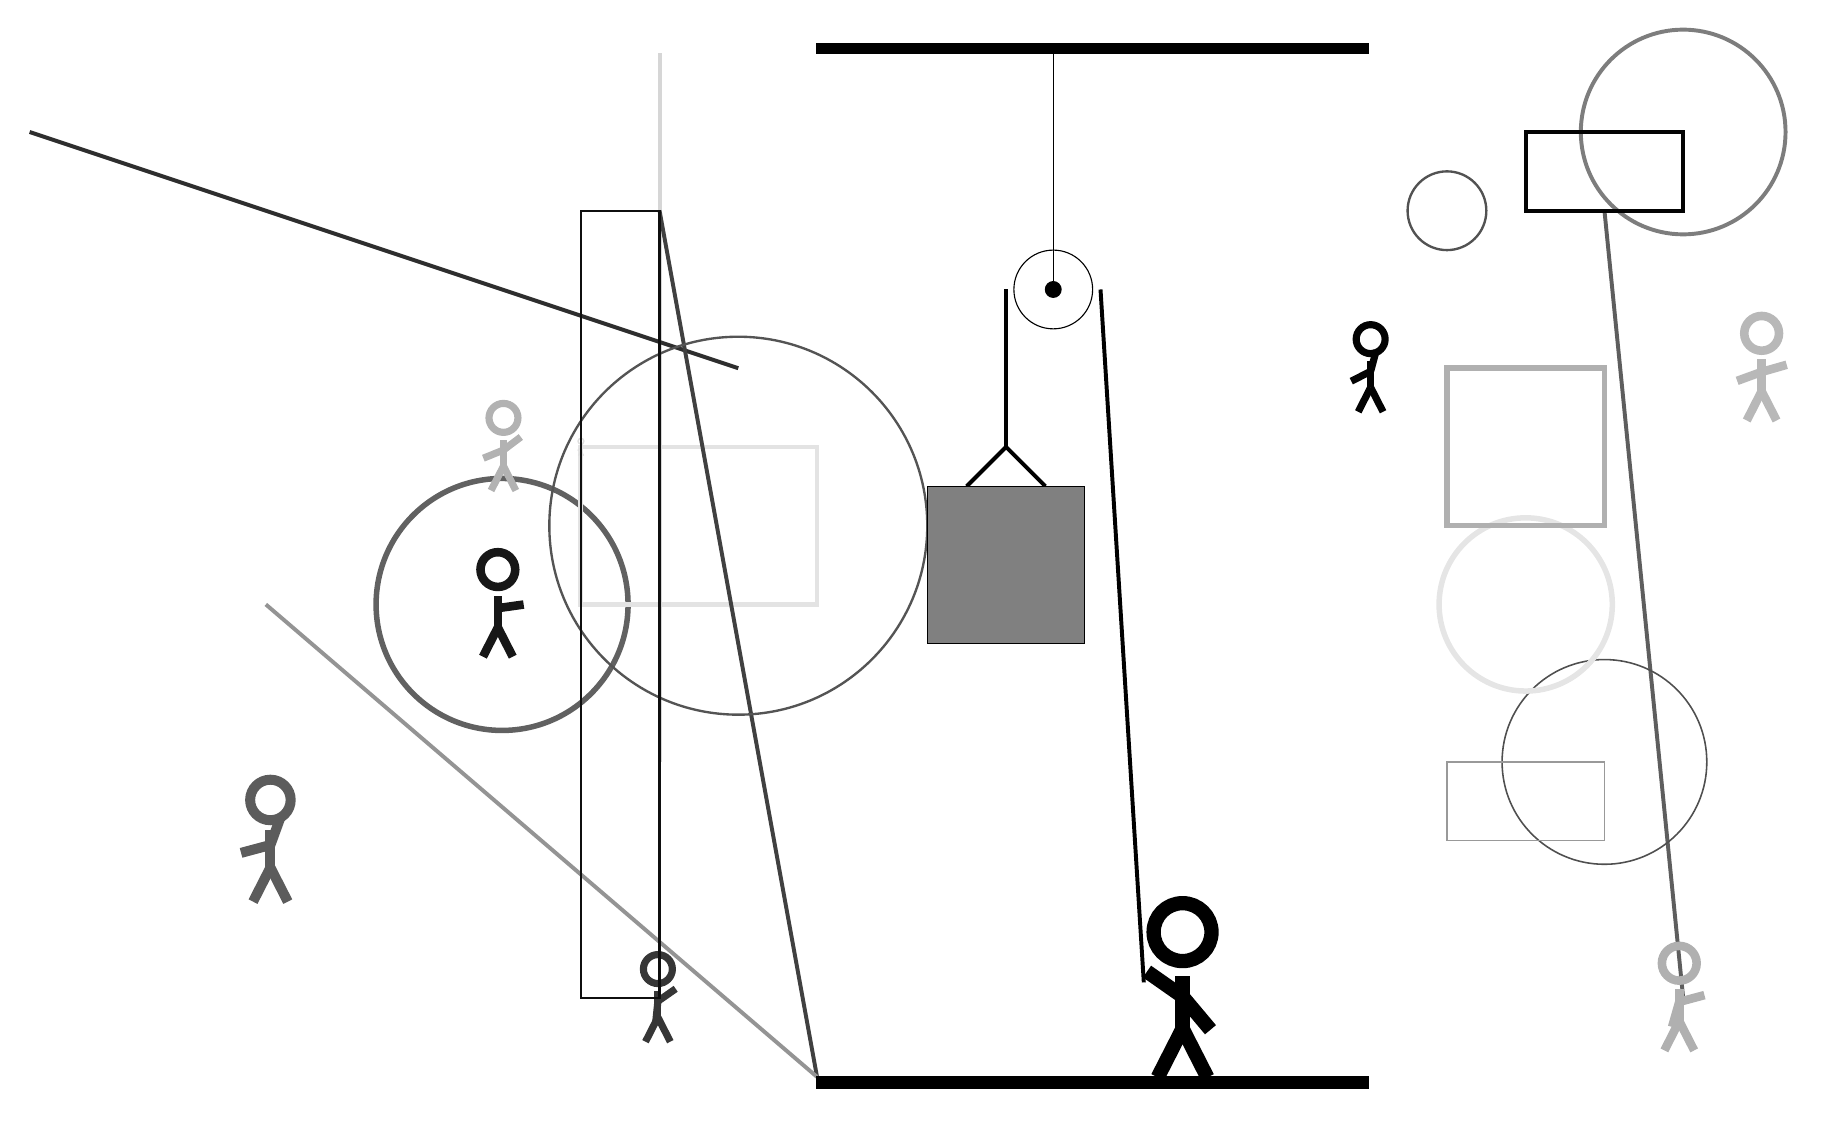
\begin{tikzpicture}
		%%%%% START %%%%%
		
		\draw[fill=black] (-2, 10) rectangle (5, 10.125);
		
		\node[line width=0.5mm, color=black!28] at (10, 6) {\Strichmaxerl[6][20][16]};
		
		\draw [line width=0.5mm, color=black!51](9, 9) circle (1.3);
		\draw [line width=0.7mm, color=black!62](-6, 3) circle (1.6);
		\draw[line width=0.6mm, color=black!11] (-2, 5) rectangle (-5, 3);
		\draw[line width=0.5mm, color=black!63](9, -2) -- (8, 8);
		
		\draw[line width=0.5mm, color=black!16](-4, 10) -- (-4, 1);
		\node[line width=0.5mm, color=black!31] at (9, -2) {\Strichmaxerl[6][74][15]};
		\draw [line width=0.2mm, color=black!69](8, 1) circle (1.3);
		\node[line width=0.7mm, color=black!64] at (-9, 0) {\Strichmaxerl[7][15][70]};
		\node[line width=0.4mm, color=black!99] at (5, 6) {\Strichmaxerl[5][27][75]};
		\draw[line width=0.2mm, color=black!40] (6, 0) rectangle (8, 1);
		\draw[line width=0.5mm, color=black!82](-3, 6) -- (-12, 9);
		\draw[line width=0.5mm, color=black!75](-4, 8) -- (-2, -3);
		
		\draw[line width=0.5mm, color=black!42](-2, -3) -- (-9, 3);
		\draw [line width=0.3mm, color=black!67](-3, 4) circle (2.4);
		\draw [line width=0.7mm, color=black!10](7, 3) circle (1.1);
		
		\node[line width=0.2mm, color=black!79] at (-4, -2) {\Strichmaxerl[5][84][35]};
		
		\draw[line width=0.5mm, color=black!99] (7, 9) rectangle (9, 8);
		\draw[line width=0.7mm, color=black!31] (6, 6) rectangle (8, 4);
		\node[line width=0.2mm, color=black!13] at (-5, 5) {\Strichmaxerl[1][43][67]};
		\draw[line width=0.3mm, color=black!94] (-4, -2) rectangle (-5, 8);
		\node[line width=0.2mm, color=black!30] at (-6, 5) {\Strichmaxerl[5][22][37]};
		\draw [line width=0.3mm, color=black!68](6, 8) circle (0.5);
		\node[line width=0.3mm, color=black!91] at (-6, 3) {\Strichmaxerl[6][90][8]};
		
		\draw (1, 7) circle (0.5);
		\draw[fill=black] (1, 7) circle (0.1);
		\draw (1, 10) -- (1, 7);
		
		\draw[line width=0.5mm] (-0.1, 4.5) -- (0.4, 5.0) -- (0.9, 4.5);
		\draw[fill=black!50] (-0.6, 4.5) rectangle (1.4, 2.5);
		
		\draw[line width=0.5mm] (0.4, 7) -- (0.4, 5.0);
		\centerarc[line width=0.5mm](1, 7)(0:180:0.6);
		\draw[line width=0.5mm](1.6, 7) -- (2.15, -1.8);
		
		\node at (2.6, -1.9) {\Strichmaxerl[10][-35][-50]};
		
		\draw[fill=black] (-2, -3) rectangle (5, -3.15);
		
		%%%%% END %%%%%
	\end{tikzpicture}
\end{document}